\begin{sidewaysfigure}[p]
\begin{subfigure}{\textwidth}
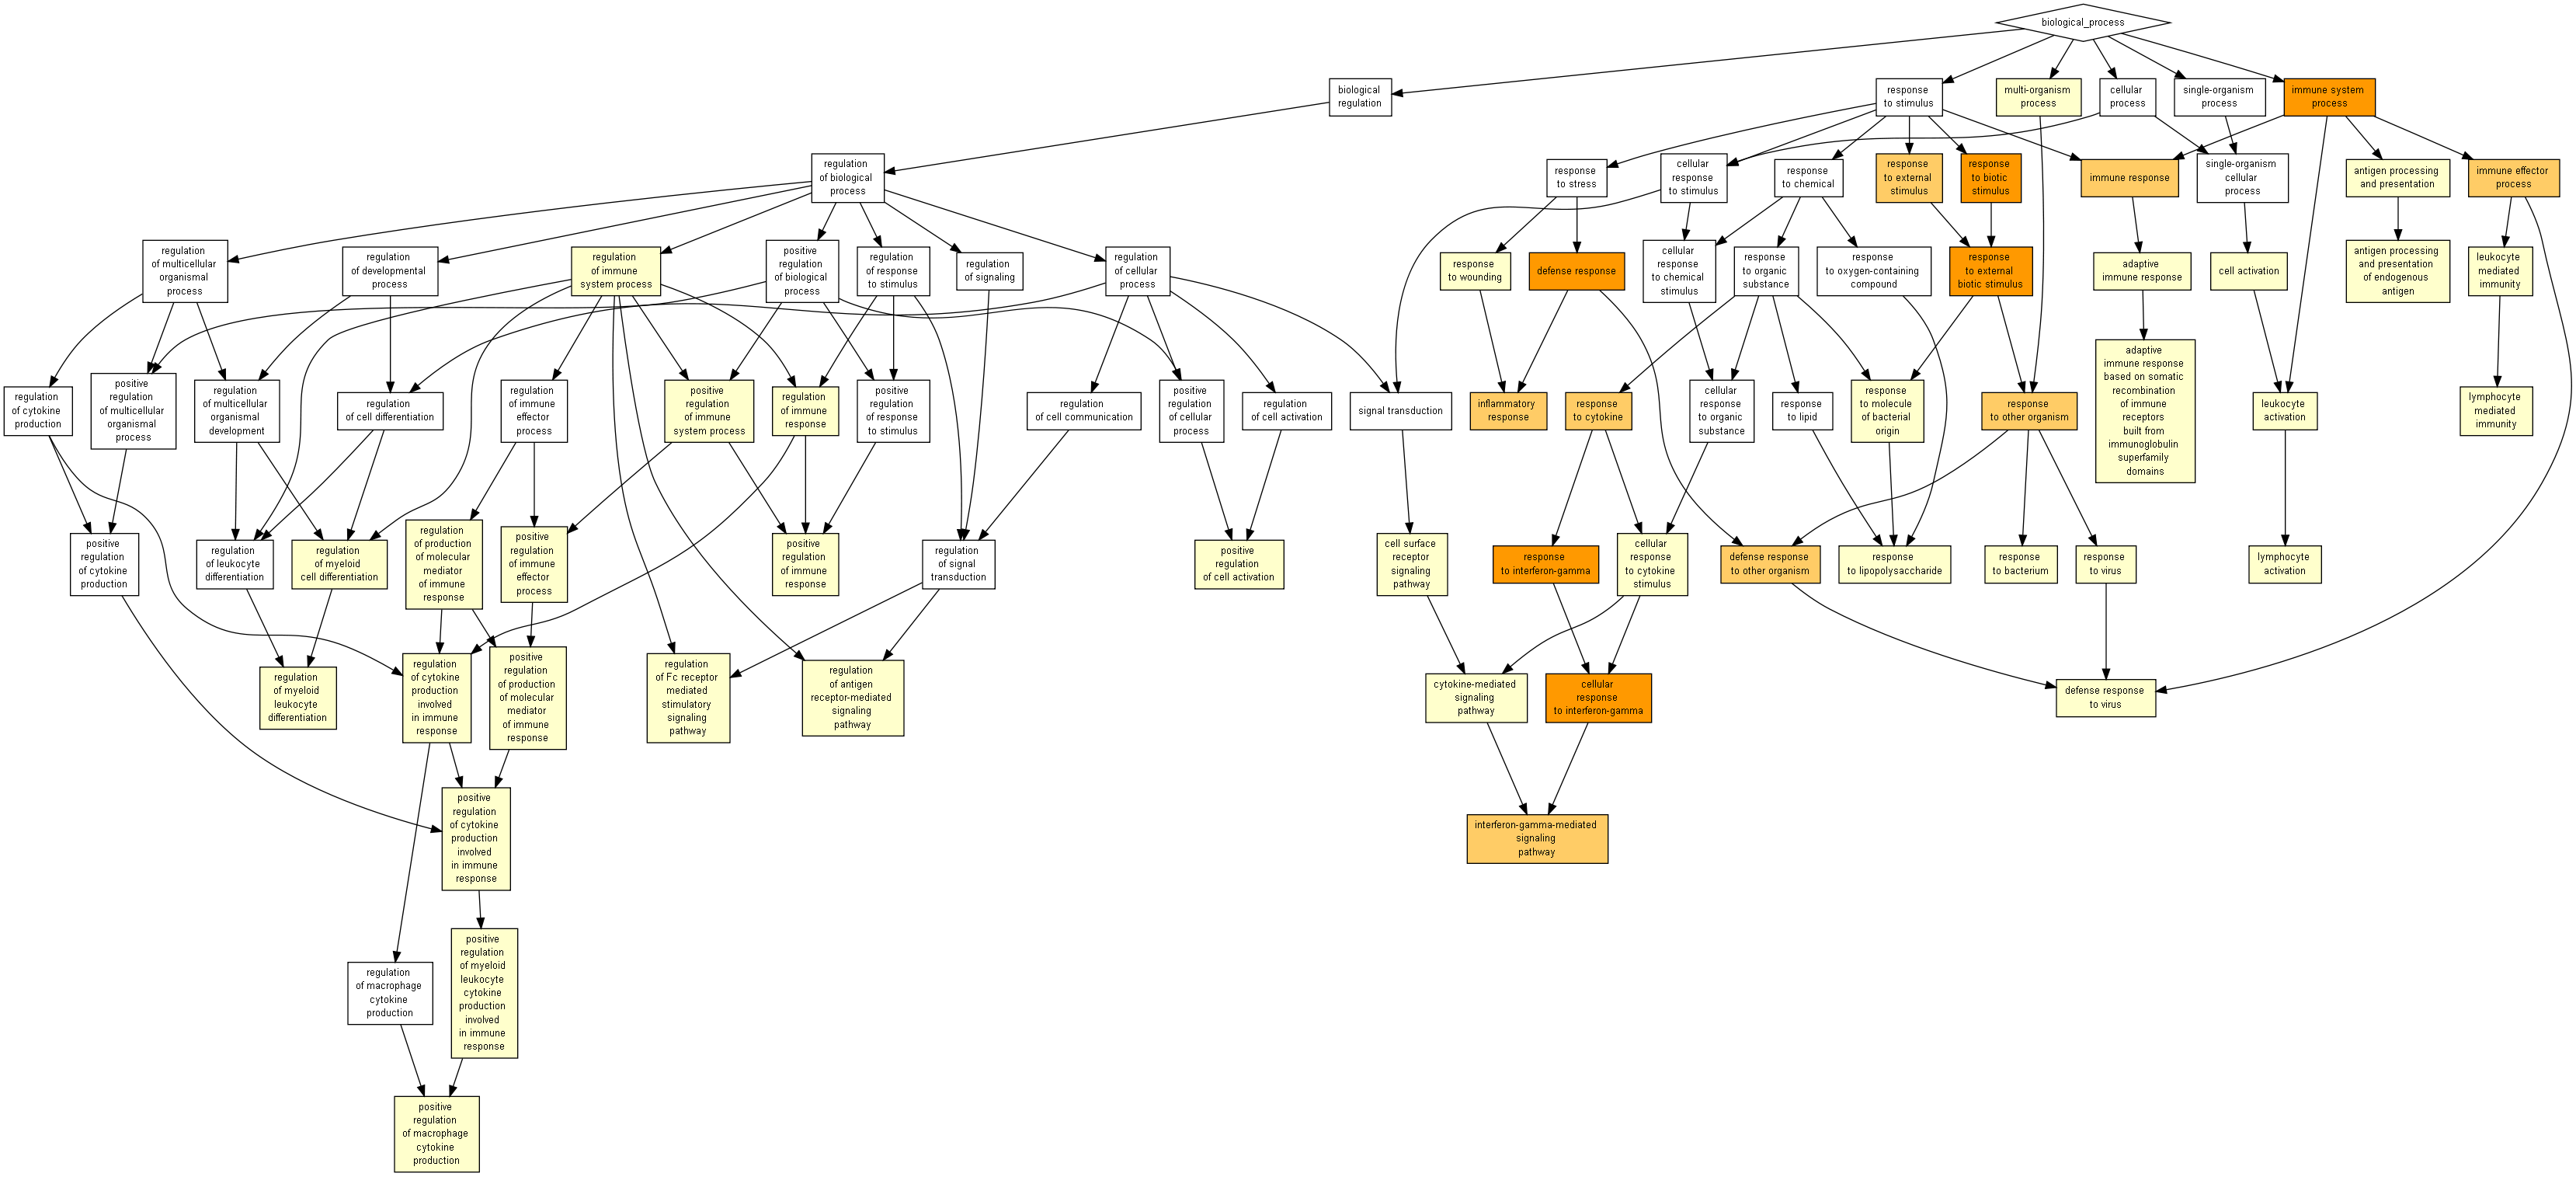
\includegraphics[width=\textwidth]
{Figures/hlc-go-pot-down/hlc-go-pot-down.png}
\caption{Vue générale}
\end{subfigure}
\end{sidewaysfigure}

\begin{figure}[p]
\ContinuedFloat
\begin{subfigure}{\textwidth}
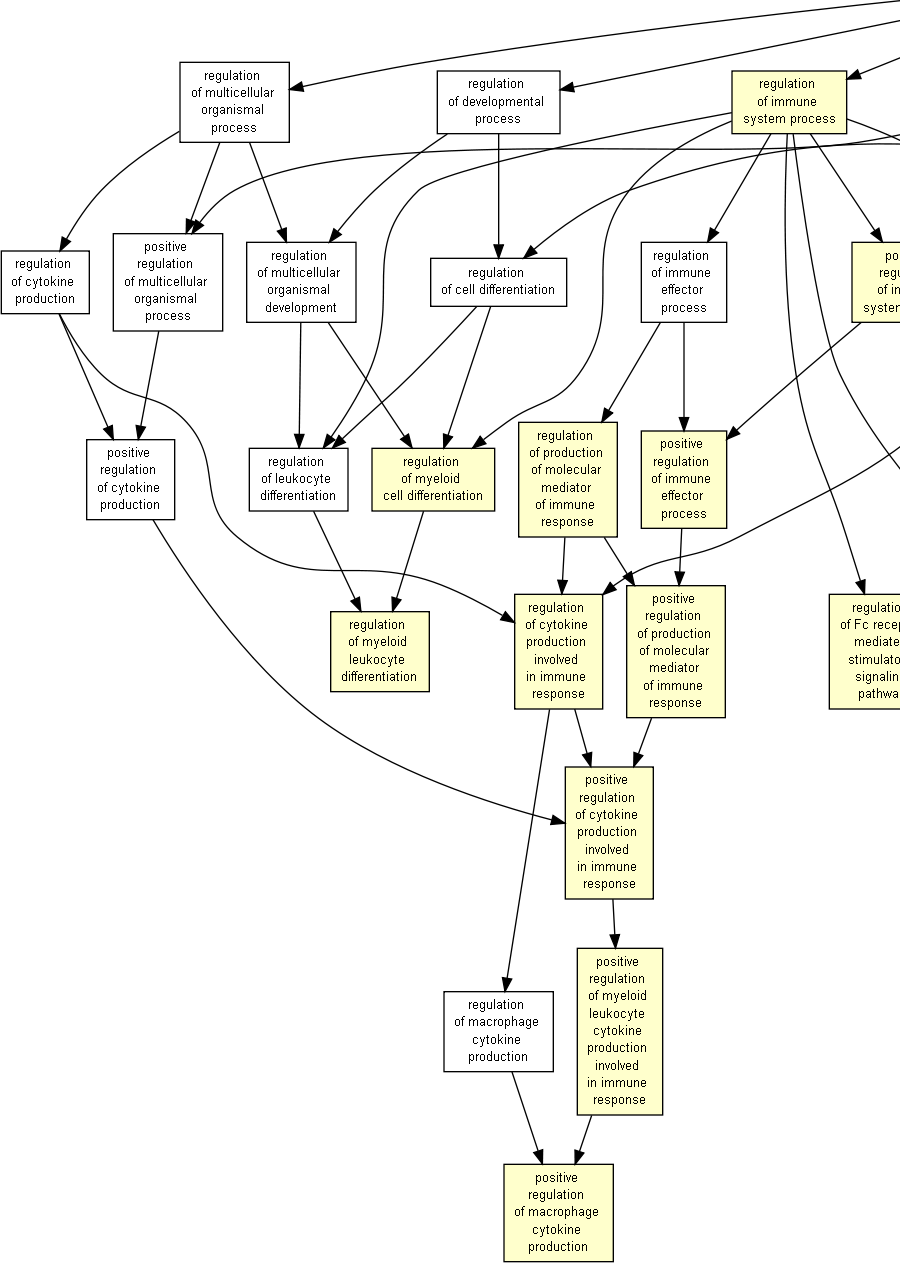
\includegraphics[width=\textwidth]
{Figures/hlc-go-pot-down/hlc-go-pot-down_0.png}
\caption{1/4}
\end{subfigure}
\end{figure}

\begin{figure}[p]
\ContinuedFloat
\begin{subfigure}{\textwidth}
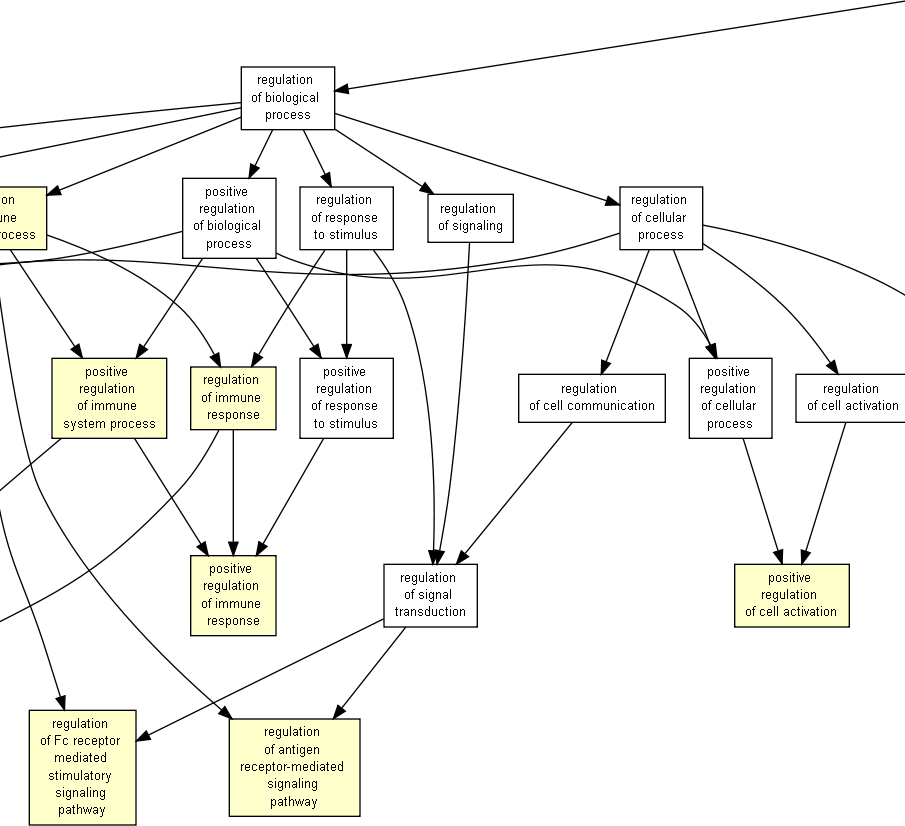
\includegraphics[width=\textwidth]
{Figures/hlc-go-pot-down/hlc-go-pot-down_1.png}
\caption{2/4}
\end{subfigure}
\end{figure}

\begin{figure}[p]
\ContinuedFloat
\begin{subfigure}{\textwidth}
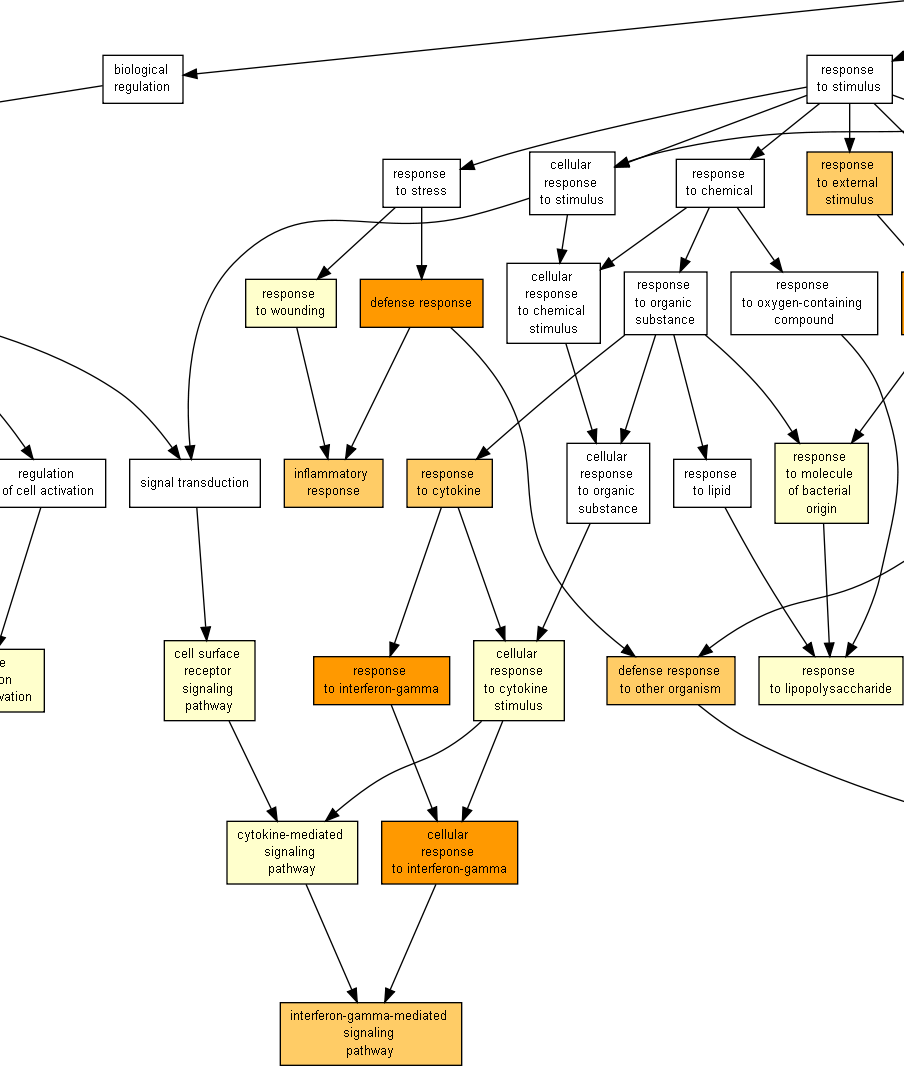
\includegraphics[width=\textwidth]
{Figures/hlc-go-pot-down/hlc-go-pot-down_2.png}
\caption{3/4}
\end{subfigure}
\end{figure}

\begin{figure}[!htp]
\ContinuedFloat
\begin{subfigure}{\textwidth}
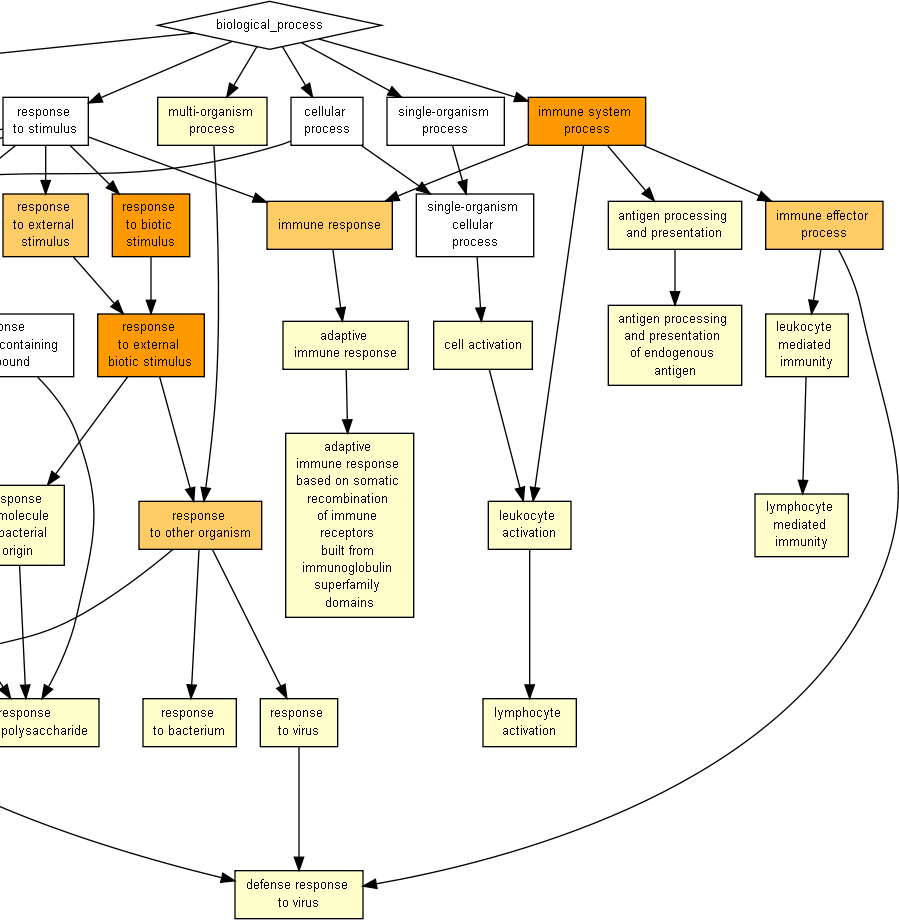
\includegraphics[width=\textwidth]
{Figures/hlc-go-pot-down/hlc-go-pot-down_3.png}
\caption{4/4}
\end{subfigure}
\caption[Enrichissement fonctionnel des gènes dont la répression \gls{t3}-dépendante est potentiée par la \gls{cort}]
{
(Cinq pages précédentes) Enrichissement fonctionnel des gènes dont la répression \gls{t3}-dépendante est potentiée par la \gls{cort}
a) Vue générale
b) Détail
L'enrichissement des termes comparé à l'ensemble des gènes transcrits est calculé à l'aide de GOrilla \citep{Eden2009}.
Les couleurs des boites correspondent à la significativité de l'enrichissement.
Jaune pâle : $10^{-3} \leq p < 10^{-5}$
Jaune : $10^{-5} \leq p < 10^{-7}$
Orange : $10^{-7} \leq p < 10^{-9}$
Rouge: $p < 10^{-9}$
}
\label{fig:hlc-go-pot-down}
\end{figure}